\documentclass{article}

% Packages
\usepackage[margin=1.5cm, includefoot, footskip=30pt]{geometry}
\usepackage{hyperref}
\usepackage{multicol}
\usepackage{booktabs}
\usepackage{xstring}
\usepackage{subcaption}
\usepackage{graphicx}
\usepackage{amsmath}
\usepackage{standalone}
\usepackage{fancyvrb}

\usepackage{pdflscape}

\usepackage{tikz}
\usetikzlibrary{calc, shapes, patterns}

\usepackage[backend=biber, firstinits=false, backref=false, url=true,
            isbn=true, style=numeric]{biblatex}
\addbibresource{bibliography.bib}

% Title
\title{Reinforcement Learning Produces Dominant Strategies for the
Iterated Prisoner's Dilemma}
\author{Marc Harper \and Vincent Knight} % TODO Authors?
\date{}


\begin{document}

\maketitle


\begin{abstract}
    We present tournament results and several powerful strategies for the Iterated
    Prisoner's Dilemma created using reinforcement learning techniques
    (evolutionary and particle swarm algorithms). These strategies are
    trained to perform well against a corpus of over 100 distinct
    opponents, including many well-known strategies from the literature, and all
    the trained strategies win standard tournaments against the total collection
    of other opponents. We also trained variants to win noisy tournaments.
\end{abstract}

\section{Introduction}\label{sec:introduction}

* Update on Axelrod Library

% TODO: more

The Axelrod library \cite{knight2016open} now contains over 200 strategies,
many from the scientific literature, including classic strategies like Win Stay
Lose Shift \cite{nowak1993strategy} and previous tournament winners such as
OmegaTFT \cite{slany2007some}, Adaptive Pavlov \cite{li2007design}, and
ZDGTFT2 \cite{stewart2012extortion}.

% TODO: discuss earlier tournaments

There are several previous publications that use evolutionary algorithms to
evolve IPD strategies in various circumstances \cite{marks1989niche} \cite{fogel1993evolving} \cite{ashlock2006training}
\cite{ashlock2006changes} \cite{vassiliades2010multiagent} \cite{ashlock2014shaped}
\cite{ashlock2014evolution} \cite{ashlock2015multiple} \cite{barlow2015varying}
\cite{sudo2015effects}. See also \cite{gaudesi2016exploiting} for a strategy
trained to win against a collection of well-known IPD opponents and see
\cite{franken2005particle} for a prior use of particle swarm algorithms. Our
results are unique in that we are able to train against a large collection of
well-known strategies available in the scientific literature.

\section{The Strategy Archetypes}

The Axelrod library now contains many strategies based on machine learning
methods. Most are deterministic, use many rounds of memory, and perform
extremely well in tournaments.

\subsection{LookerUp}

The first strategy trained with reinforcement learning in the library is based
on lookup tables. The strategy encodes a set of deterministic responses
based on the opponent's first $n_1$ moves, the opponent's last $m_1$ moves, and
the players last $m_2$ moves. If $n_1 > 0$ then the player has infinite memory
depth, otherwise it has depth $\max{m_1, m_2}$. Although we tried various
combinations of $n_1, m_1,$ and $m_2$, the best performance at the time of
training was obtained for $n_1 = m_1 = m_2 = 2$ and generally for $n_1 > 0$.
First impressions matter in the IPD. The library includes a strategy
called EvolvedLookerUp2\_2\_2 which is among the top strategies in the library.

This archetype can be used to train deterministic memory-$n$ strategies with the
parameters $n_1=0$ and $m_1=m_2=n$. For $n=1$, the resulting strategy cooperates
if the last round was mutual cooperation and defects otherwise.

Two strategies in the library, Winner12 and Winner21, from \cite{Mathieu2015},
are based on lookup tables for $n_1 = 0$, $m_1 = 1$, and $m_2=2$. The strategy
Winner12 emerged in less than 10 generations of training in our framework using
a score maximizing objective. Strategies nearly identical to Winner21 arise
from training with a Moran process objective.

\subsection{PSO Gambler}

PSO Gambler is a stochastic variant of LookerUp. Instead of deterministically
encoded moves the lookup table emits probabilities which are
used to choose cooperation or defection. The library includes a player trained
with $n_1 = m_1 = m_2 = 2$ that is \emph{mostly deterministic}, with most of the
probabilities being 0 or 1. At one time this strategy outperformed
EvolvedLookerUp2\_2\_2.

This strategy type can be used to train arbitrary memory-$n$ strategies and a
memory one strategy was trained and is called PSO Gambler Mem 1, with
probabilities $(\text{Pr(C|CC)}, \text{Pr(C|CD)}, \text{Pr(C|DC)}, \text{Pr(C|DD)}) = (1, 0.5217, 0, 0.121)$. Though it performs well in deterministic tournaments
it is not as good as the longer memory strategies, and is bested by a similar
strategy that also uses the first round of play.

These strategies are trained with a particle swarm algorithm rather than an
evolutionary algorithm (though the former would suffice). Particle swarm
algorithms have been used to trained IPD strategies previously
\cite{franken2005particle}.

% TODO: quantify how stochastic

\subsection{ANN: Single Layer Artificial Neural Network}

Strategies based on artificial neural networks can also be trained with an
evolutionary algorithm. A variety of features are computed from the history
of play such as the opponents trailing moves, the total number of cooperations
of the player and the opponent, and several others, which are then input
into a feed forward neural network with one layer and user-supplied width.
An inner layer with just five nodes performs quite well in both deterministic and
noisy tournaments. The output of the ANN used in this work is deterministic and
a stochastic variant that outputs probabilities rather than exact moves could
be easily created.

% TODO: list features

\subsection{Finite State Machines}

We used strategies based on finite state machines to create a number of
strategies. These strategies are deterministic and are efficient computational.
At each state the machine transitions to a new state and plays a specified move
depending on the opponent's last action. These strategies can encode a variety
of other strategies, including classic strategies like TitForTat, encode
handshakes, and grudging strategies that always defect after an opponent
defection.

% TODO: One or more FSM diagrams

\subsection{Hidden Markov Models}

We also trained stochastic versions of finite state machine players called
hidden Markov model players or HMMs. These strategies also encode an internal
state with probabilistic transitions to other states and cooperate or defect
with various probabilities at each state. These are the best performing
stochastic strategies in the library but take longer to train due to their
stochasticity.

\subsection{Meta Strategies}

Last but not least there are several strategies based on ensemble methods that
are common in machine learning called Meta strategies. These strategies are
composed of a team of other strategies and each is polled for its desired next
move. The ensemble then selects the next move based on some rule, such as the
consensus vote in the case of MetaMajority or the best individual performance
in the case of MetaWinner. These strategies were among the best in the library
before the inclusion of those trained by reinforcement learning.

Because these strategies inherit many of the properties of the strategies
on which they are based, including using the match length to defect on the last
rounds of play, these strategies were omitted from the tournament results.

\section{Results}

\subsection{Standard Tournament}

We conducted a tournament with all strategies in the Axelrod library, including
some parametrized strategies. These are listed in
Appendix~\ref{app:list_of_players}.
% TODO Add list of players
The top
11 performing strategies by median payoff are all strategies trained to maximize
% TODO Potentially modify this as more repetitions are analysed.
total payoff against a subset of the strategies (Table~\ref{tbl:standard_score}).
The next strategy is
Desired Belief Strategy (DBS)
% TODO Add reference for DBS
which actively analyzes the opponent and responds
accordingly. The next two strategies are Winner12, based on a lookup table,
Fool Me Once, a grudging strategy that defects indefinitely on
the second defection and Omega Tit For Tat.
% TODO Add a reference for Omega TfT
All strategies in the tournament follow a simple set of
rules in accordance with earlier tournaments:

\begin{itemize}
  \item Players are unaware of the number of turns in a match
  \item Players carry no acquired state between matches
  \item Players cannot observe the outcome of other matches
  \item Players cannot identify their opponent by any label or identifier
  \item Players cannot manipulate or inspect their opponents in any way
\end{itemize}

% Table of best strategies
\begin{table}[!hbtp]
    \centering
        \begin{tabular}{lrrrrrrrrr}
\toprule
{} &   mean &    std &    min &     5\% &    25\% &    50\% &    75\% &    95\% &    max \\
\midrule
EvolvedLookerUp2\_2\_2    &  2.955 &  0.010 &  2.915 &  2.937 &  2.948 &  2.956 &  2.963 &  2.971 &  2.984 \\
Evolved HMM 5           &  2.954 &  0.014 &  2.903 &  2.931 &  2.945 &  2.954 &  2.964 &  2.977 &  3.003 \\
Evolved FSM 16          &  2.952 &  0.013 &  2.900 &  2.930 &  2.944 &  2.953 &  2.962 &  2.973 &  2.993 \\
PSO Gambler 2\_2\_2       &  2.938 &  0.013 &  2.886 &  2.913 &  2.930 &  2.940 &  2.948 &  2.957 &  2.971 \\
Evolved FSM 16 Noise 05 &  2.919 &  0.013 &  2.874 &  2.898 &  2.910 &  2.919 &  2.928 &  2.940 &  2.961 \\
PSO Gambler 1\_1\_1       &  2.912 &  0.023 &  2.810 &  2.873 &  2.896 &  2.912 &  2.927 &  2.950 &  3.012 \\
Evolved ANN 5           &  2.912 &  0.010 &  2.873 &  2.894 &  2.905 &  2.912 &  2.919 &  2.928 &  2.944 \\
Evolved FSM 4           &  2.910 &  0.012 &  2.868 &  2.889 &  2.901 &  2.910 &  2.919 &  2.929 &  2.942 \\
Evolved ANN             &  2.907 &  0.010 &  2.865 &  2.891 &  2.901 &  2.908 &  2.914 &  2.923 &  2.942 \\
PSO Gambler Mem1        &  2.901 &  0.025 &  2.794 &  2.859 &  2.884 &  2.902 &  2.919 &  2.942 &  2.984 \\
Evolved ANN 5 Noise 05  &  2.864 &  0.008 &  2.837 &  2.850 &  2.858 &  2.865 &  2.870 &  2.877 &  2.891 \\
DBS: 0.75, 3, 4, 3, 5   &  2.857 &  0.009 &  2.827 &  2.842 &  2.851 &  2.857 &  2.863 &  2.872 &  2.888 \\
Winner12                &  2.849 &  0.008 &  2.821 &  2.836 &  2.843 &  2.850 &  2.855 &  2.862 &  2.873 \\
Fool Me Once            &  2.844 &  0.008 &  2.820 &  2.831 &  2.838 &  2.844 &  2.850 &  2.857 &  2.882 \\
Omega TFT: 3, 8         &  2.841 &  0.011 &  2.805 &  2.822 &  2.833 &  2.841 &  2.849 &  2.859 &  2.878 \\
\bottomrule
\end{tabular}

        \caption{Standard Tournament: Top Ranking Strategies by median score
        (50th percentile) in 15,000 Tournaments}
        % TODO Update caption as more repetitions are carried out
        % TODO Potentially remove count from table (including it for now so as
        % to avoid confusion.
        \label{tbl:standard_score}
\end{table}

Violin plots showing the distribution of the scores of each strategy (again
ranked by median score) are shown in Figure~\ref{fig:standard_boxplot}.

\begin{landscape}
    \begin{figure}[!hbtp]
        \includegraphics[width=\paperwidth]{./assets/standard_scores_boxplots.pdf}
        \caption{Ranking by median score for the Standard Tournament}
        \label{fig:standard_boxplot}
    \end{figure}
\end{landscape}

Pairwise payoff results are given as a heatmap (Figure~\ref{fig:standard_heatmap})
which shows that many strategies achieve mutual cooperation with each other and
that the top performing strategies never defect first but are able to exploit
weaker strategies that attempt to defect.

\begin{figure}[!hbtp]
    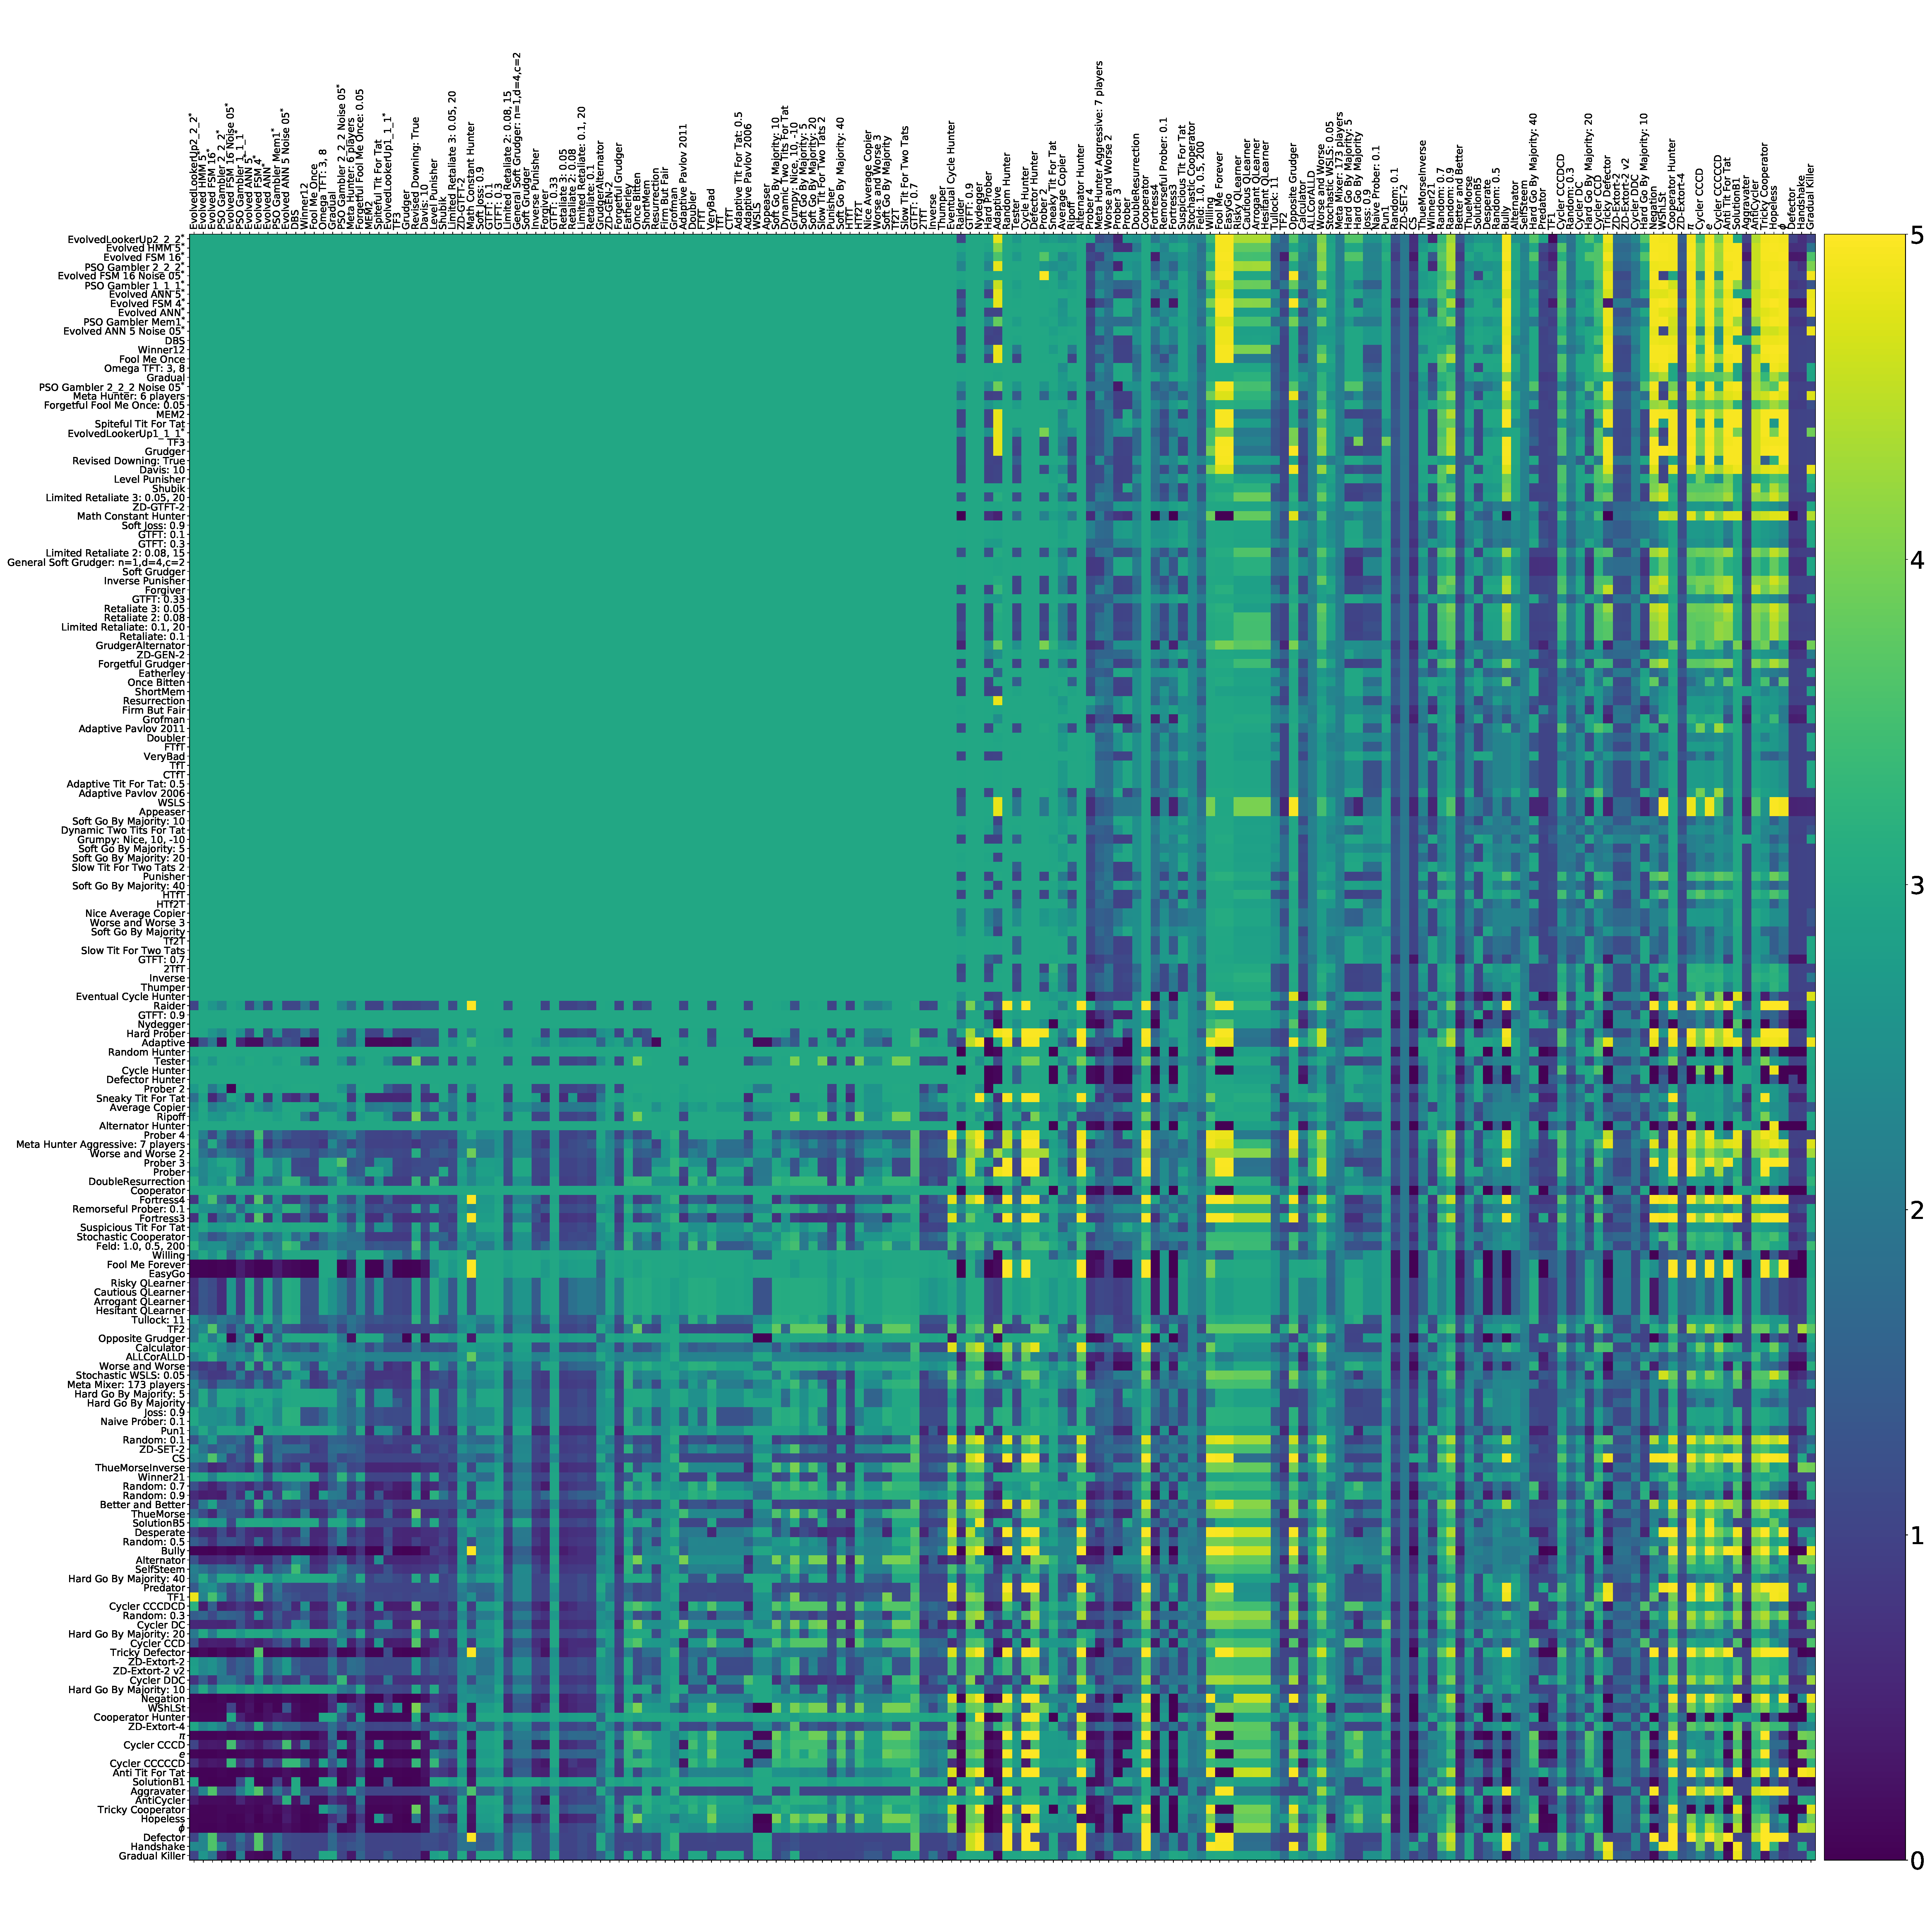
\includegraphics[width=\textwidth]{./assets/standard_scores_heatmap.pdf}
    \caption{Pairwise Match results for the Standard Tournament}
    \label{fig:standard_heatmap}
\end{figure}

The strategies that win the most matches are Defector, Aggravater, followed by
handshaking and zero determinant strategies. This includes two handshaking
strategies that were the result of training to maximize Moran process fixation.
No strategies were trained specifically to win matches.
None of the top scoring
strategies appear in the top 20 list of strategies ranked by match wins.
This can be seen in Figure~\ref{fig:standard_winplot} where the distribution of
the number of wins of each strategy is shown.

\begin{landscape}
    \begin{figure}[!hbtp]
        \centering
        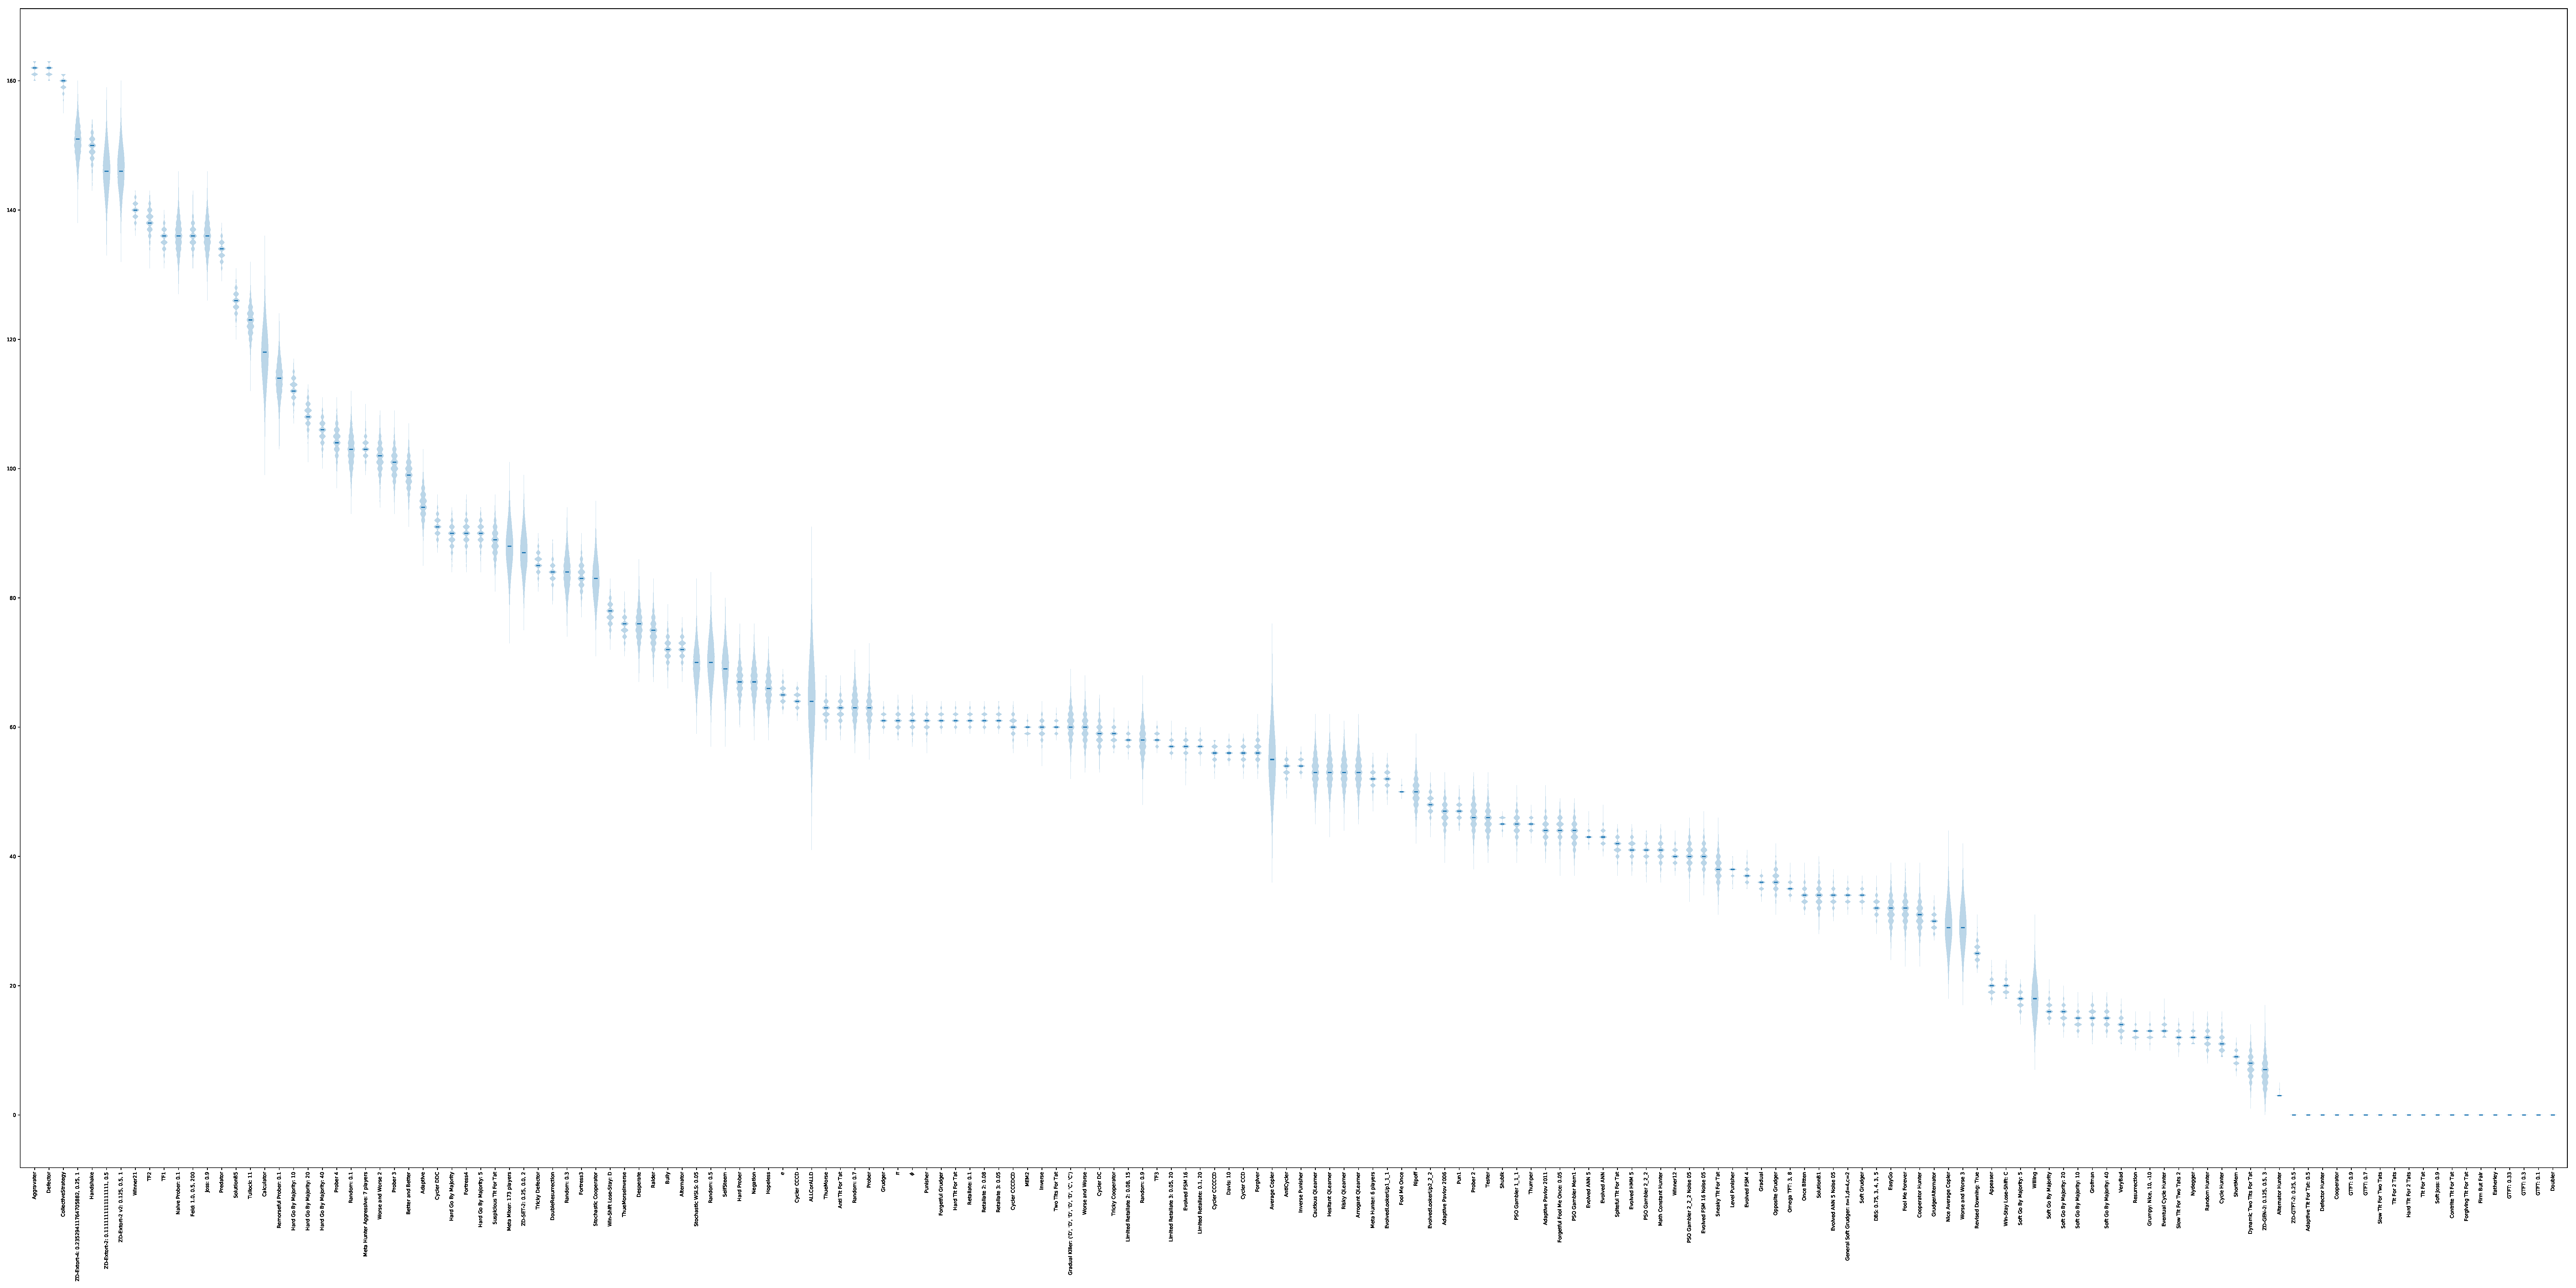
\includegraphics[width=\textwidth]{./assets/standard_wins_boxplots.pdf}
        \caption{Ranking by Total wins for the Standard Tournament}
        \label{fig:standard_winplot}
    \end{figure}
\end{landscape}

The number of wins of the top strategies of Table~\ref{tbl:standard_wins} are
shown in Table~\ref{tbl:standard_wins}. It is evident that although these
strategies score highly they do not win many matches: the strategy with the most
number of wins is the Evolved FSM 16 strategy that at most won 60
(\(60/175\approx34\%\)) matches in a given tournament.
% TODO Update this when more data comes in.

\begin{table}[!hbtp]
    \centering
        \begin{tabular}{lrrrrrrrrrr}
\toprule
{} &  count &    mean &    std &  min &    5\% &   25\% &   50\% &   75\% &   95\% &  max \\
\midrule
EvolvedLookerUp2\_2\_2    &  15000 &  48.262 &  1.335 &   43 &  46.0 &  47.0 &  48.0 &  49.0 &  50.0 &   53 \\
Evolved HMM 5           &  15000 &  41.349 &  1.225 &   37 &  39.0 &  41.0 &  41.0 &  42.0 &  43.0 &   45 \\
Evolved FSM 16          &  15000 &  56.973 &  1.102 &   51 &  55.0 &  56.0 &  57.0 &  58.0 &  59.0 &   60 \\
PSO Gambler 2\_2\_2       &  15000 &  40.677 &  1.085 &   36 &  39.0 &  40.0 &  41.0 &  41.0 &  42.0 &   44 \\
Evolved FSM 16 Noise 05 &  15000 &  40.075 &  1.677 &   34 &  37.0 &  39.0 &  40.0 &  41.0 &  43.0 &   47 \\
PSO Gambler 1\_1\_1       &  15000 &  44.980 &  1.597 &   39 &  42.0 &  44.0 &  45.0 &  46.0 &  48.0 &   51 \\
Evolved ANN 5           &  15000 &  43.222 &  0.674 &   41 &  42.0 &  43.0 &  43.0 &  44.0 &  44.0 &   47 \\
Evolved FSM 4           &  15000 &  37.230 &  0.951 &   35 &  36.0 &  37.0 &  37.0 &  38.0 &  39.0 &   41 \\
Evolved ANN             &  15000 &  43.108 &  1.021 &   40 &  42.0 &  42.0 &  43.0 &  44.0 &  45.0 &   48 \\
PSO Gambler Mem1        &  15000 &  43.466 &  1.831 &   37 &  40.0 &  42.0 &  44.0 &  45.0 &  46.0 &   49 \\
Evolved ANN 5 Noise 05  &  15000 &  33.707 &  1.123 &   30 &  32.0 &  33.0 &  34.0 &  34.0 &  35.0 &   38 \\
DBS: 0.75, 3, 4, 3, 5   &  15000 &  32.328 &  1.200 &   28 &  30.0 &  32.0 &  32.0 &  33.0 &  34.0 &   37 \\
Winner12                &  15000 &  40.175 &  1.041 &   37 &  39.0 &  39.0 &  40.0 &  41.0 &  42.0 &   44 \\
Fool Me Once            &  15000 &  50.123 &  0.422 &   49 &  50.0 &  50.0 &  50.0 &  50.0 &  51.0 &   52 \\
Omega TFT: 3, 8         &  15000 &  35.158 &  0.860 &   33 &  34.0 &  35.0 &  35.0 &  36.0 &  37.0 &   39 \\
\bottomrule
\end{tabular}

        \caption{Standard Tournament: Number of wins of Top Ranking Strategies
        by median score (50th percentile) in 15,000 Tournaments}
        % TODO Update caption as more repetitions are carried out
        % TODO Potentially remove count from table (including it for now so as
        % to avoid confusion.
        \label{tbl:standard_wins}
\end{table}

Finally, Table~\ref{tbl:standard_ranks} and
Figure~\ref{fig:standard_ranks_boxplot} show the ranks (based on median score)
of each strategy over the repeated tournaments. Whilst there is some
stochasticity, the top three strategies almost always rank in the top three. For
example, the worst that the Evolved Lookerup 2 2 2 ranks in a given tournament
is 7th.


\begin{table}[!hbtp]
    \centering
        \begin{tabular}{lrrrrrrrrr}
\toprule
{} &    mean &    std &  min &    5\% &   25\% &   50\% &   75\% &   95\% &  max \\
\midrule
EvolvedLookerUp2\_2\_2$^{*}$    &   2.171 &  1.069 &    1 &   1.0 &   1.0 &   2.0 &   3.0 &   4.0 &    8 \\
Evolved HMM 5$^{*}$           &   2.325 &  1.275 &    1 &   1.0 &   1.0 &   2.0 &   3.0 &   5.0 &   10 \\
Evolved FSM 16$^{*}$          &   2.488 &  1.299 &    1 &   1.0 &   1.0 &   2.0 &   3.0 &   5.0 &   10 \\
PSO Gambler 2\_2\_2$^{*}$       &   3.961 &  1.527 &    1 &   2.0 &   3.0 &   4.0 &   5.0 &   7.0 &   10 \\
Evolved FSM 16 Noise 05$^{*}$ &   6.298 &  1.688 &    1 &   4.0 &   5.0 &   6.0 &   7.0 &   9.0 &   11 \\
PSO Gambler 1\_1\_1$^{*}$       &   7.091 &  2.504 &    1 &   3.0 &   5.0 &   7.0 &   9.0 &  10.0 &   17 \\
Evolved ANN 5$^{*}$           &   7.285 &  1.524 &    2 &   5.0 &   6.0 &   7.0 &   8.0 &  10.0 &   11 \\
Evolved FSM 4$^{*}$           &   7.521 &  1.630 &    2 &   5.0 &   6.0 &   8.0 &   9.0 &  10.0 &   12 \\
Evolved ANN$^{*}$             &   7.899 &  1.450 &    2 &   5.0 &   7.0 &   8.0 &   9.0 &  10.0 &   12 \\
PSO Gambler Mem1$^{*}$        &   8.223 &  2.534 &    1 &   4.0 &   6.0 &   9.0 &  10.0 &  12.0 &   20 \\
Evolved ANN 5 Noise 05$^{*}$  &  11.362 &  0.872 &    8 &  10.0 &  11.0 &  11.0 &  12.0 &  13.0 &   16 \\
DBS                           &  12.191 &  1.121 &    9 &  11.0 &  11.0 &  12.0 &  13.0 &  14.0 &   16 \\
Winner12                      &  13.224 &  1.136 &    9 &  11.0 &  12.0 &  13.0 &  14.0 &  15.0 &   17 \\
Fool Me Once                  &  13.961 &  1.080 &    9 &  12.0 &  13.0 &  14.0 &  15.0 &  15.0 &   17 \\
Omega TFT: 3, 8               &  14.274 &  1.300 &    9 &  12.0 &  13.0 &  15.0 &  15.0 &  16.0 &   19 \\
\bottomrule
\end{tabular}

        \caption{Standard Tournament: Ranks of Top Ranking Strategies
        by median score (50th percentile) in 15,000 Tournaments}
        % TODO Update caption as more repetitions are carried out
        % TODO Potentially remove count from table (including it for now so as
        % to avoid confusion.
        \label{tbl:standard_ranks}
\end{table}

\begin{landscape}
    \begin{figure}[!hbtp]
        \centering
        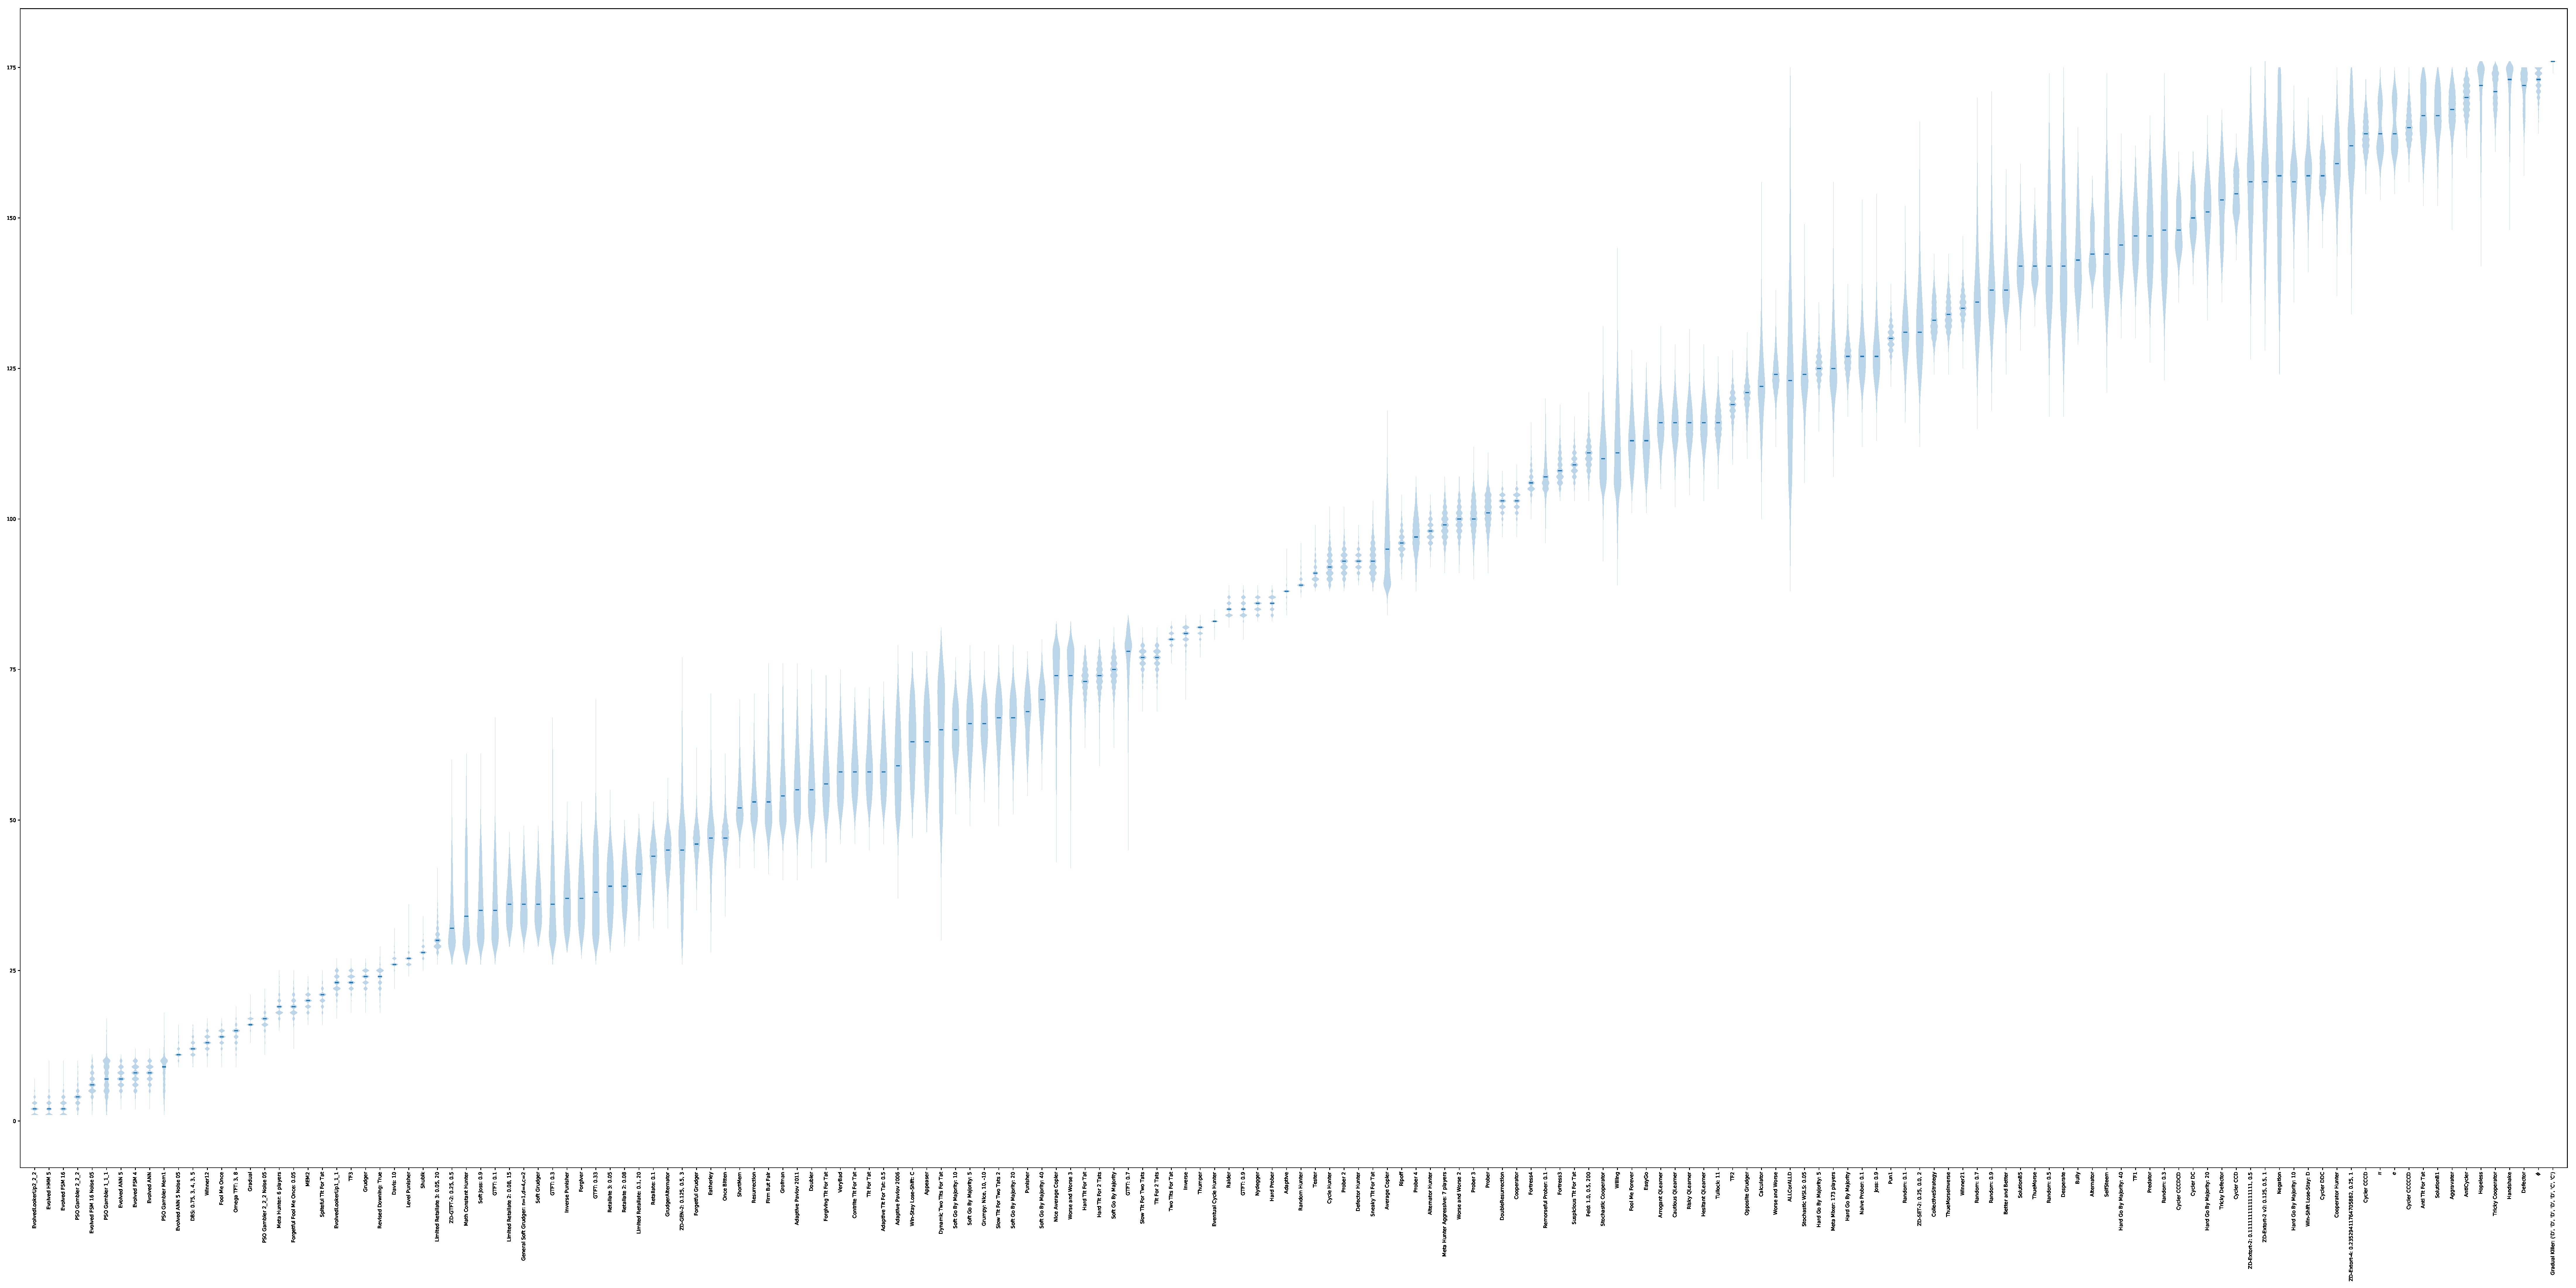
\includegraphics[width=\textwidth]{./assets/standard_ranks_boxplots.pdf}
        \caption{Rankings over each repeated tournament}
        \label{fig:standard_ranks_boxplot}
    \end{figure}
\end{landscape}


Using the method of fingerprinting described in \cite{ashlock2008fingerprinting}
% TODO This is actually a numerical approximation of the fingerprinting
% described in ashlock's paper. There they consider a fingerprint to be an
% analytic function.
\cite{ashlock2009fingerprint}, we can compare
strategies. For the top performing noisy strategies there is a striking similarity
in the fingerprints.

\begin{figure}[!hbtp]
    \centering
    \begin{subfigure}[t]{.3\textwidth}
        \centering
        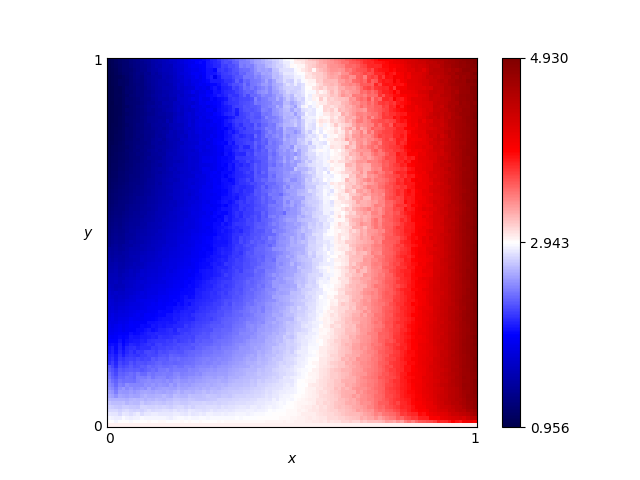
\includegraphics[width=\textwidth]{./plots/EvolvedLookerUp2_2_2.png}
        \caption{Fingerprint for EvolvedLookerUp\_2\_2\_2}
    \end{subfigure}%
    ~
    \begin{subfigure}[t]{.3\textwidth}
        \centering
        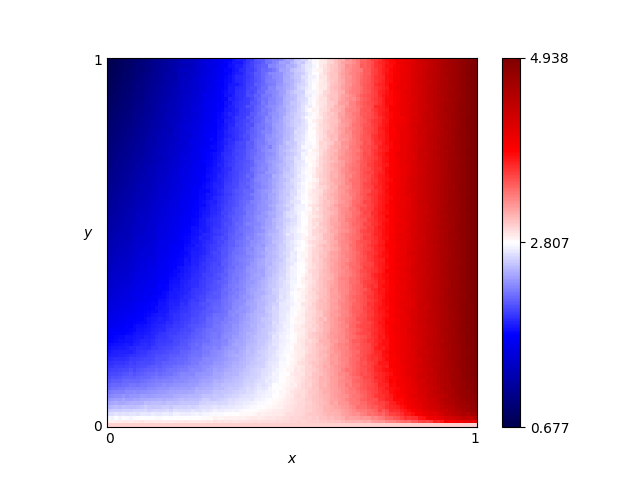
\includegraphics[width=\textwidth]{./plots/Evolved_HMM_5.png}
        \caption{Fingerprint for Evolved\_HMM\_5}
    \end{subfigure}%
    ~
    \begin{subfigure}[t]{.3\textwidth}
        \centering
        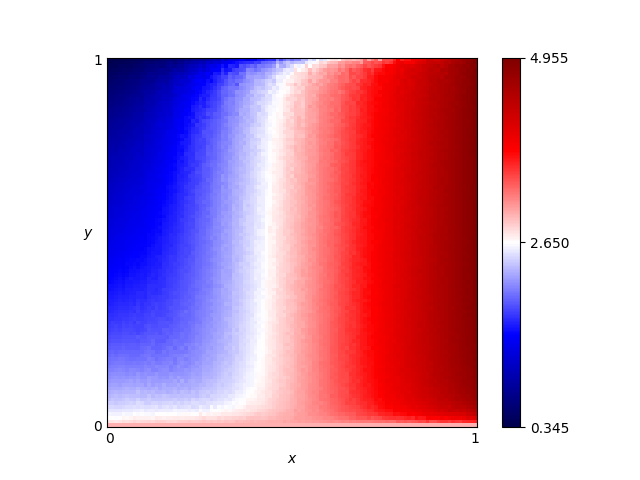
\includegraphics[width=\textwidth]{./plots/Evolved_FSM_16.png}
        \caption{Fingerprint for Evolved\_FSM\_16}
    \end{subfigure}%

    \caption{Comparison of Fingerprints for Noisy Tournament Top 3}
    \label{fig:comparison_fingerprint_noisy}
\end{figure}


\subsection{Noisy Tournament}

We also ran noisy tournaments in which there is a 10\% chance that an action
is flipped. The best performing strategies in mean payoff are DBS, designed
to correct for noise, followed by two strategies trained
in the presence of noise, Spiteful TFT (TFT but defects indefinitely if the
opponent defects twice consecutively), two strategies trained without noise, then
OmegaTFT (also designed to handle noise).

The strategies trained in the presence of noise are also among the best performers
in the absence of noise. The cluster of mutually cooperative strategies is
broken by the noise at 5\%. A similar collection of players excels at winning
matches but again they have a poor total payoff.

The strategies tallying the most wins are somewhat similar, with Defector, the
handshaking CollectiveStrategy, and Aggravate appearing as the top three again,
followed by Spiteful TFT and strategies designed to be retaliatory. Players ranked
12, 13, and 15 (TF3, Fool Me Once, and Evolved ANN 5) all appear in the top 15
strategies by score, indicating that noise breaks the asymmetry between wins
and scores to some extent.

% Table of best strategies

\begin{table}[!hbtp]
    \centering
        \begin{tabular}{llr}
\toprule
Rank & Player &  Median Score \\
\midrule
1 & DBS: 0.75, 3, 4, 3, 5 &   2.4658 \\
2 & Evolved ANN 5 Noise 05 &  2.4052\\
3 & Evolved FSM 16 Noise 05 & 2.3709\\
4 & Spiteful Tit For Tat &    2.3500\\
5 & Evolved ANN &             2.3375\\
6 & Evolved ANN 5 &           2.3321\\
7 & Omega TFT: 3, 8 &         2.3160\\
8 & Fool Me Once &            2.3159\\
9 & MEM2 &                    2.3141\\
10 & Math Constant Hunter &   2.3133\\
11 & Adaptive &               2.3051\\
12 & Hard Prober &            2.3046\\
13 & Davis: 10 &              2.3040\\
14 & Grudger &                2.3036\\
15 & TF3 &                    2.3006\\
16 & Meta Hunter: 6 players & 2.2991\\
\bottomrule
\end{tabular}

        \caption{Noisy Tournament: Top Ranking Strategies by Median Score in a
        15000 Tournaments with 10\% noise}
        \label{tbl:noisy_score}
\end{table}


\begin{landscape}
    \begin{figure}[!hbtp]
        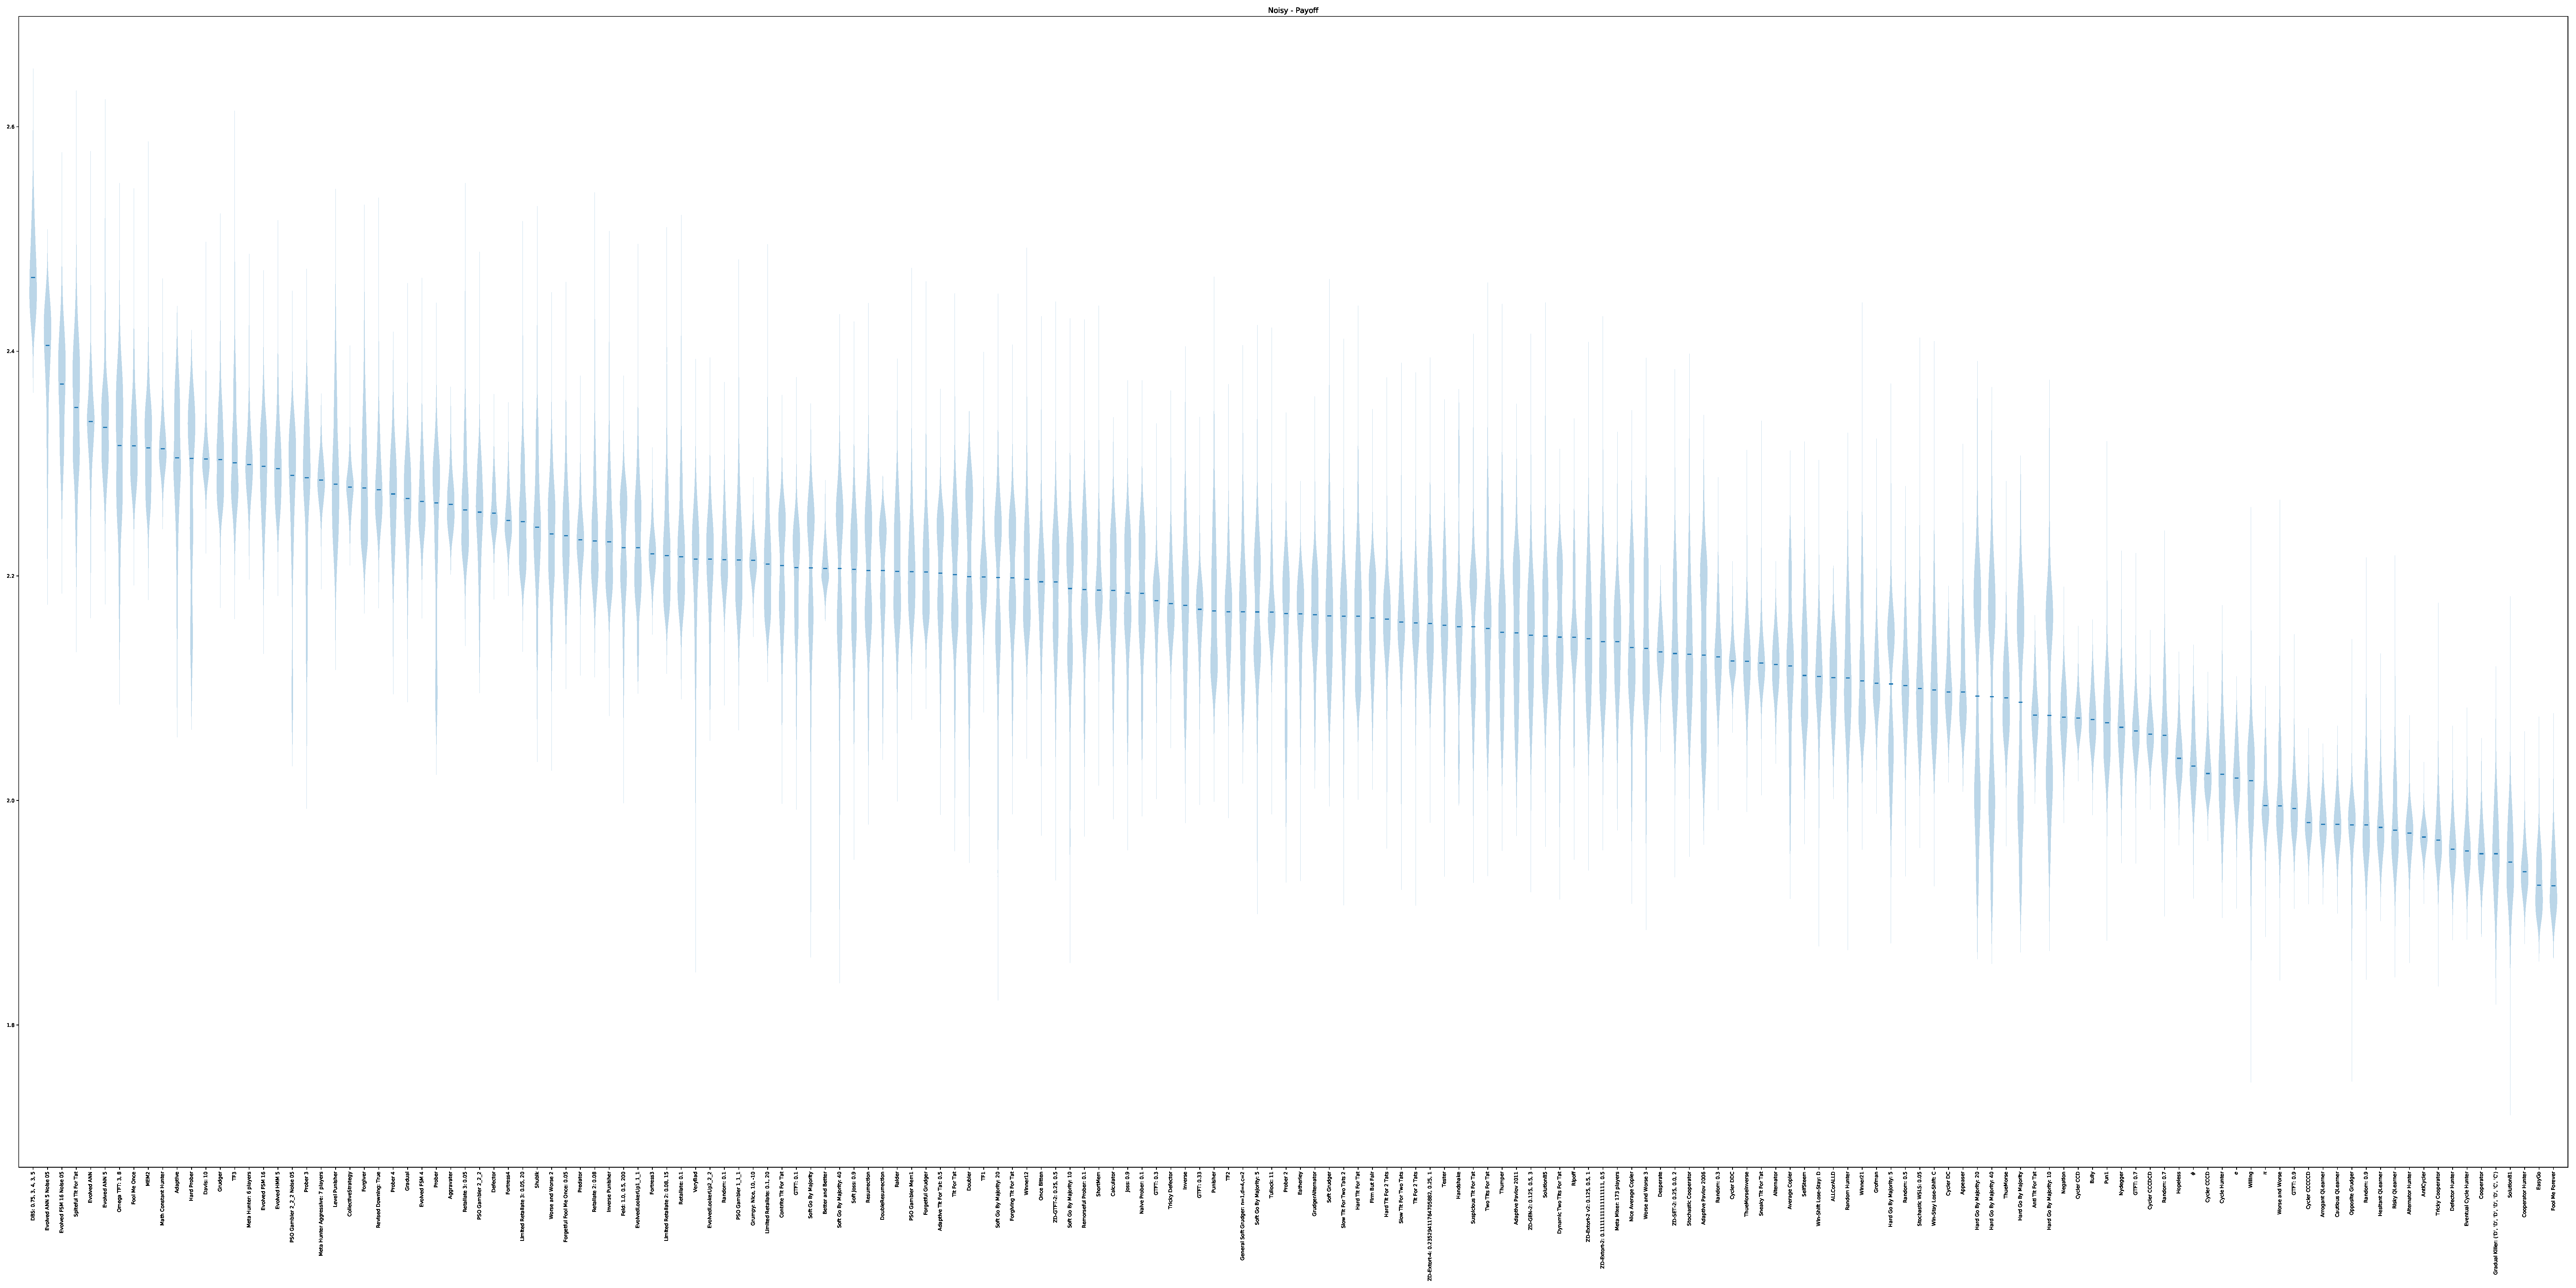
\includegraphics[width=\paperwidth]{plots/Noisy_boxplot.pdf}
        \caption{Ranking by Median Payoff for the Noisy Tournament}
    \end{figure}
\end{landscape}

\begin{landscape}
    \begin{figure}[!hbtp]
        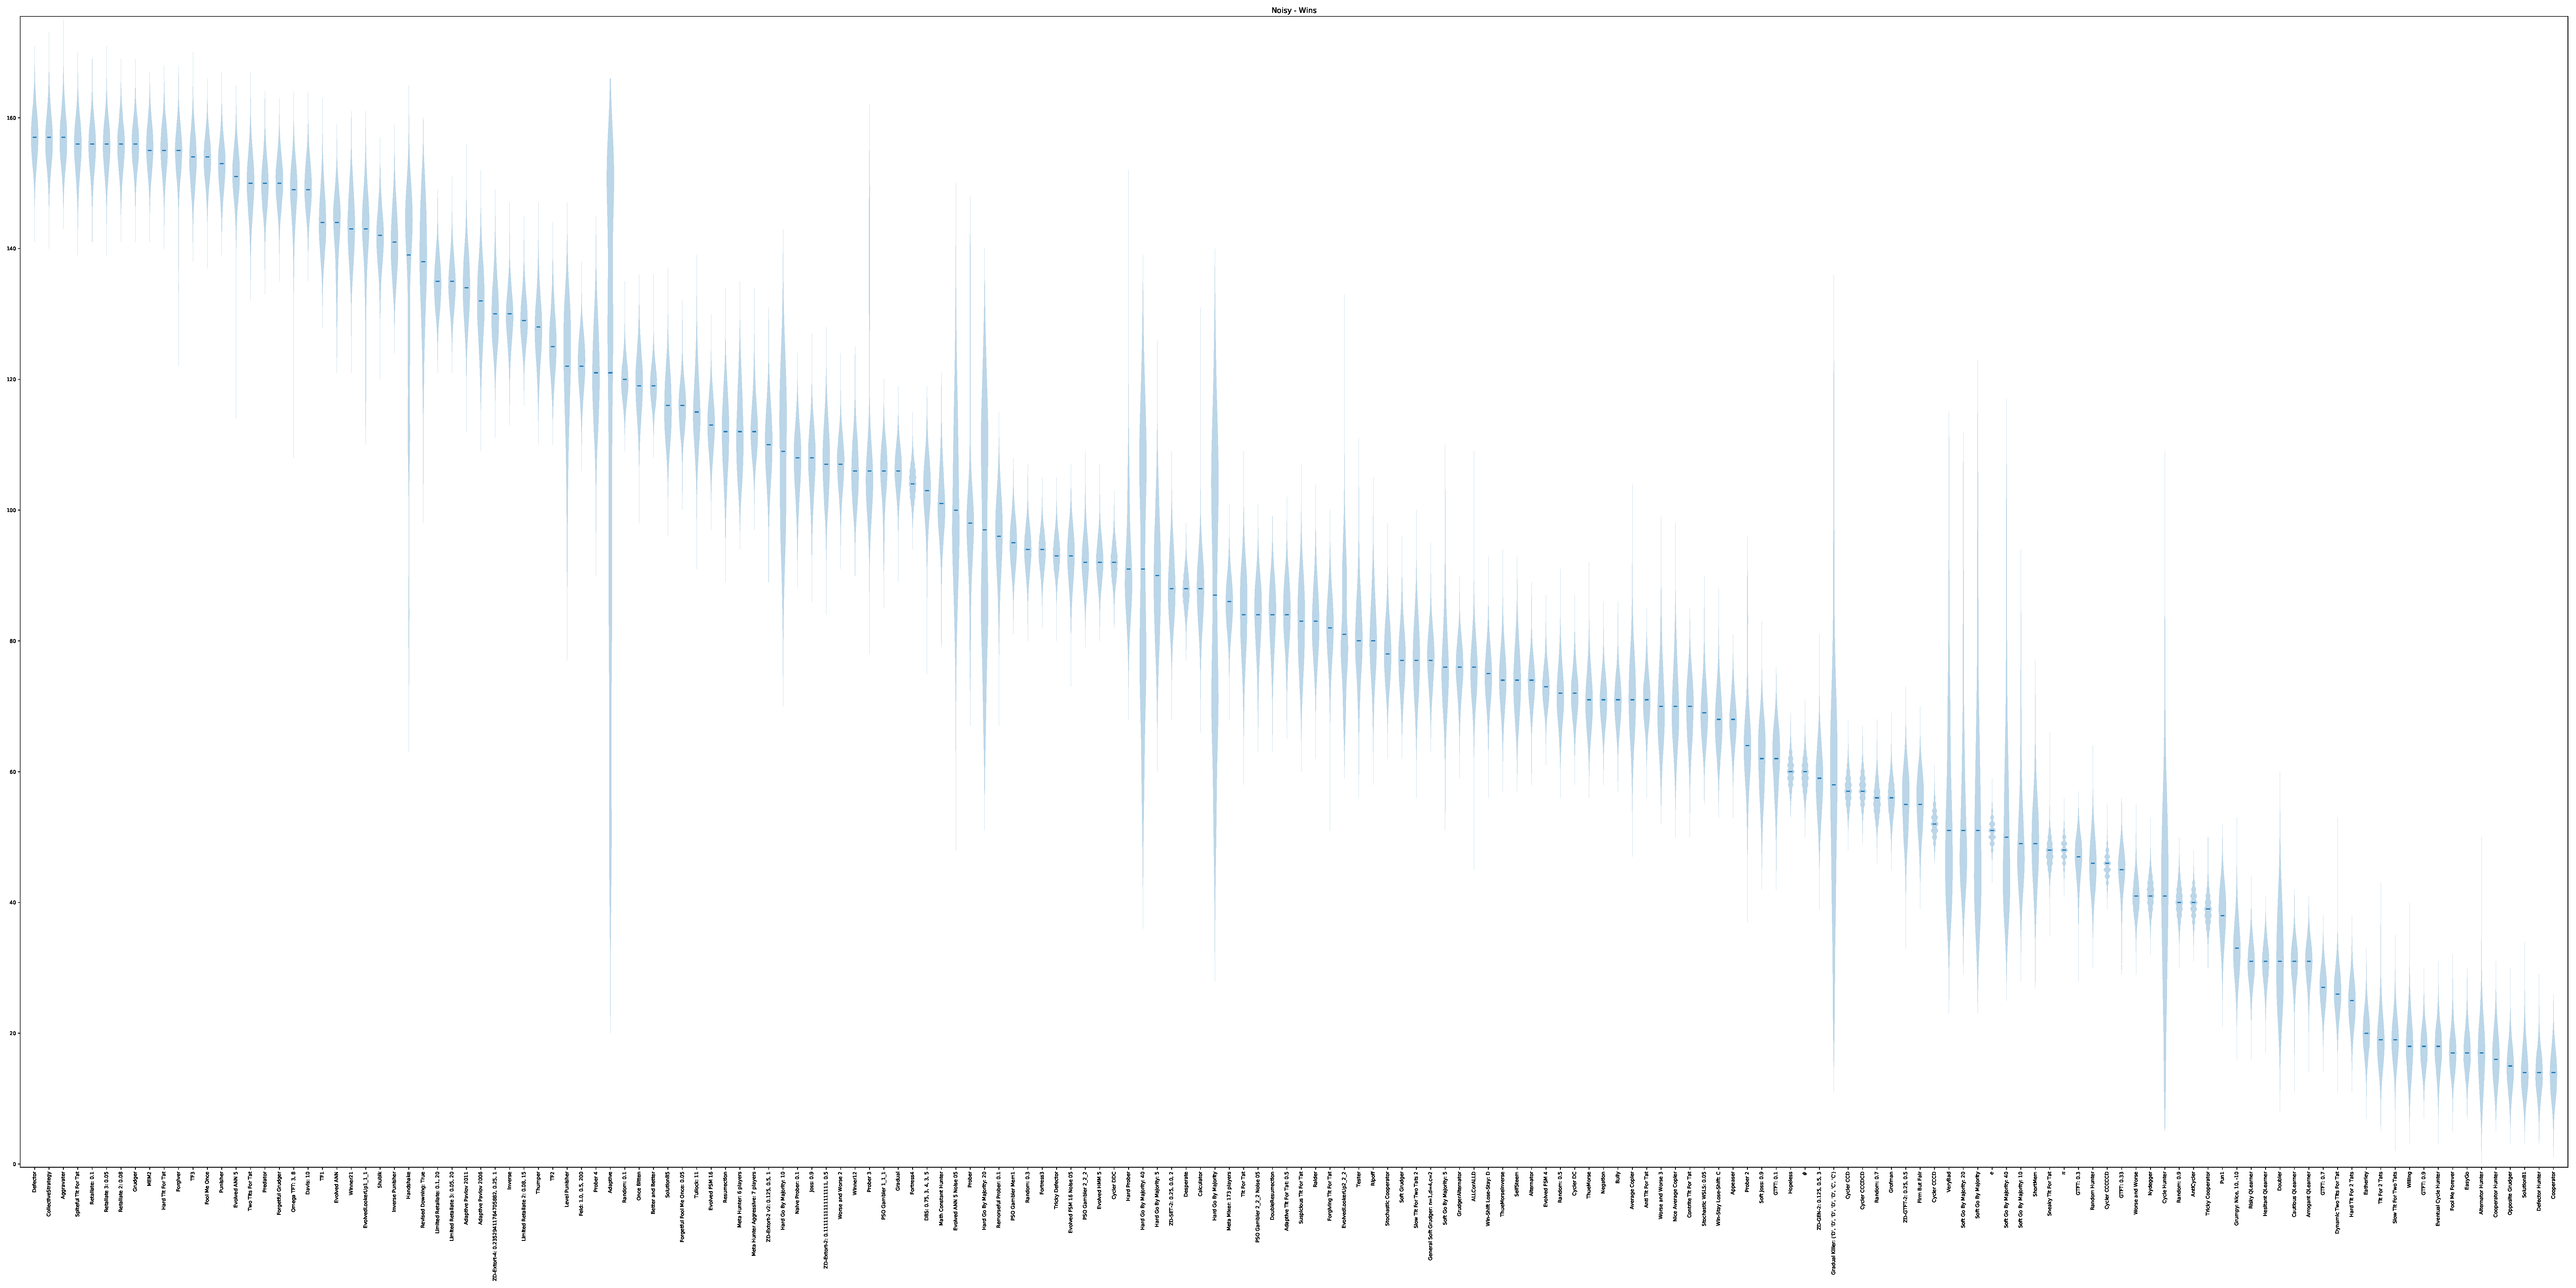
\includegraphics[width=\paperwidth]{plots/Noisy_winplot.pdf}
        \caption{Ranking by Total wins for the Noisy Tournament}
    \end{figure}
\end{landscape}

\begin{figure}[!hbtp]
    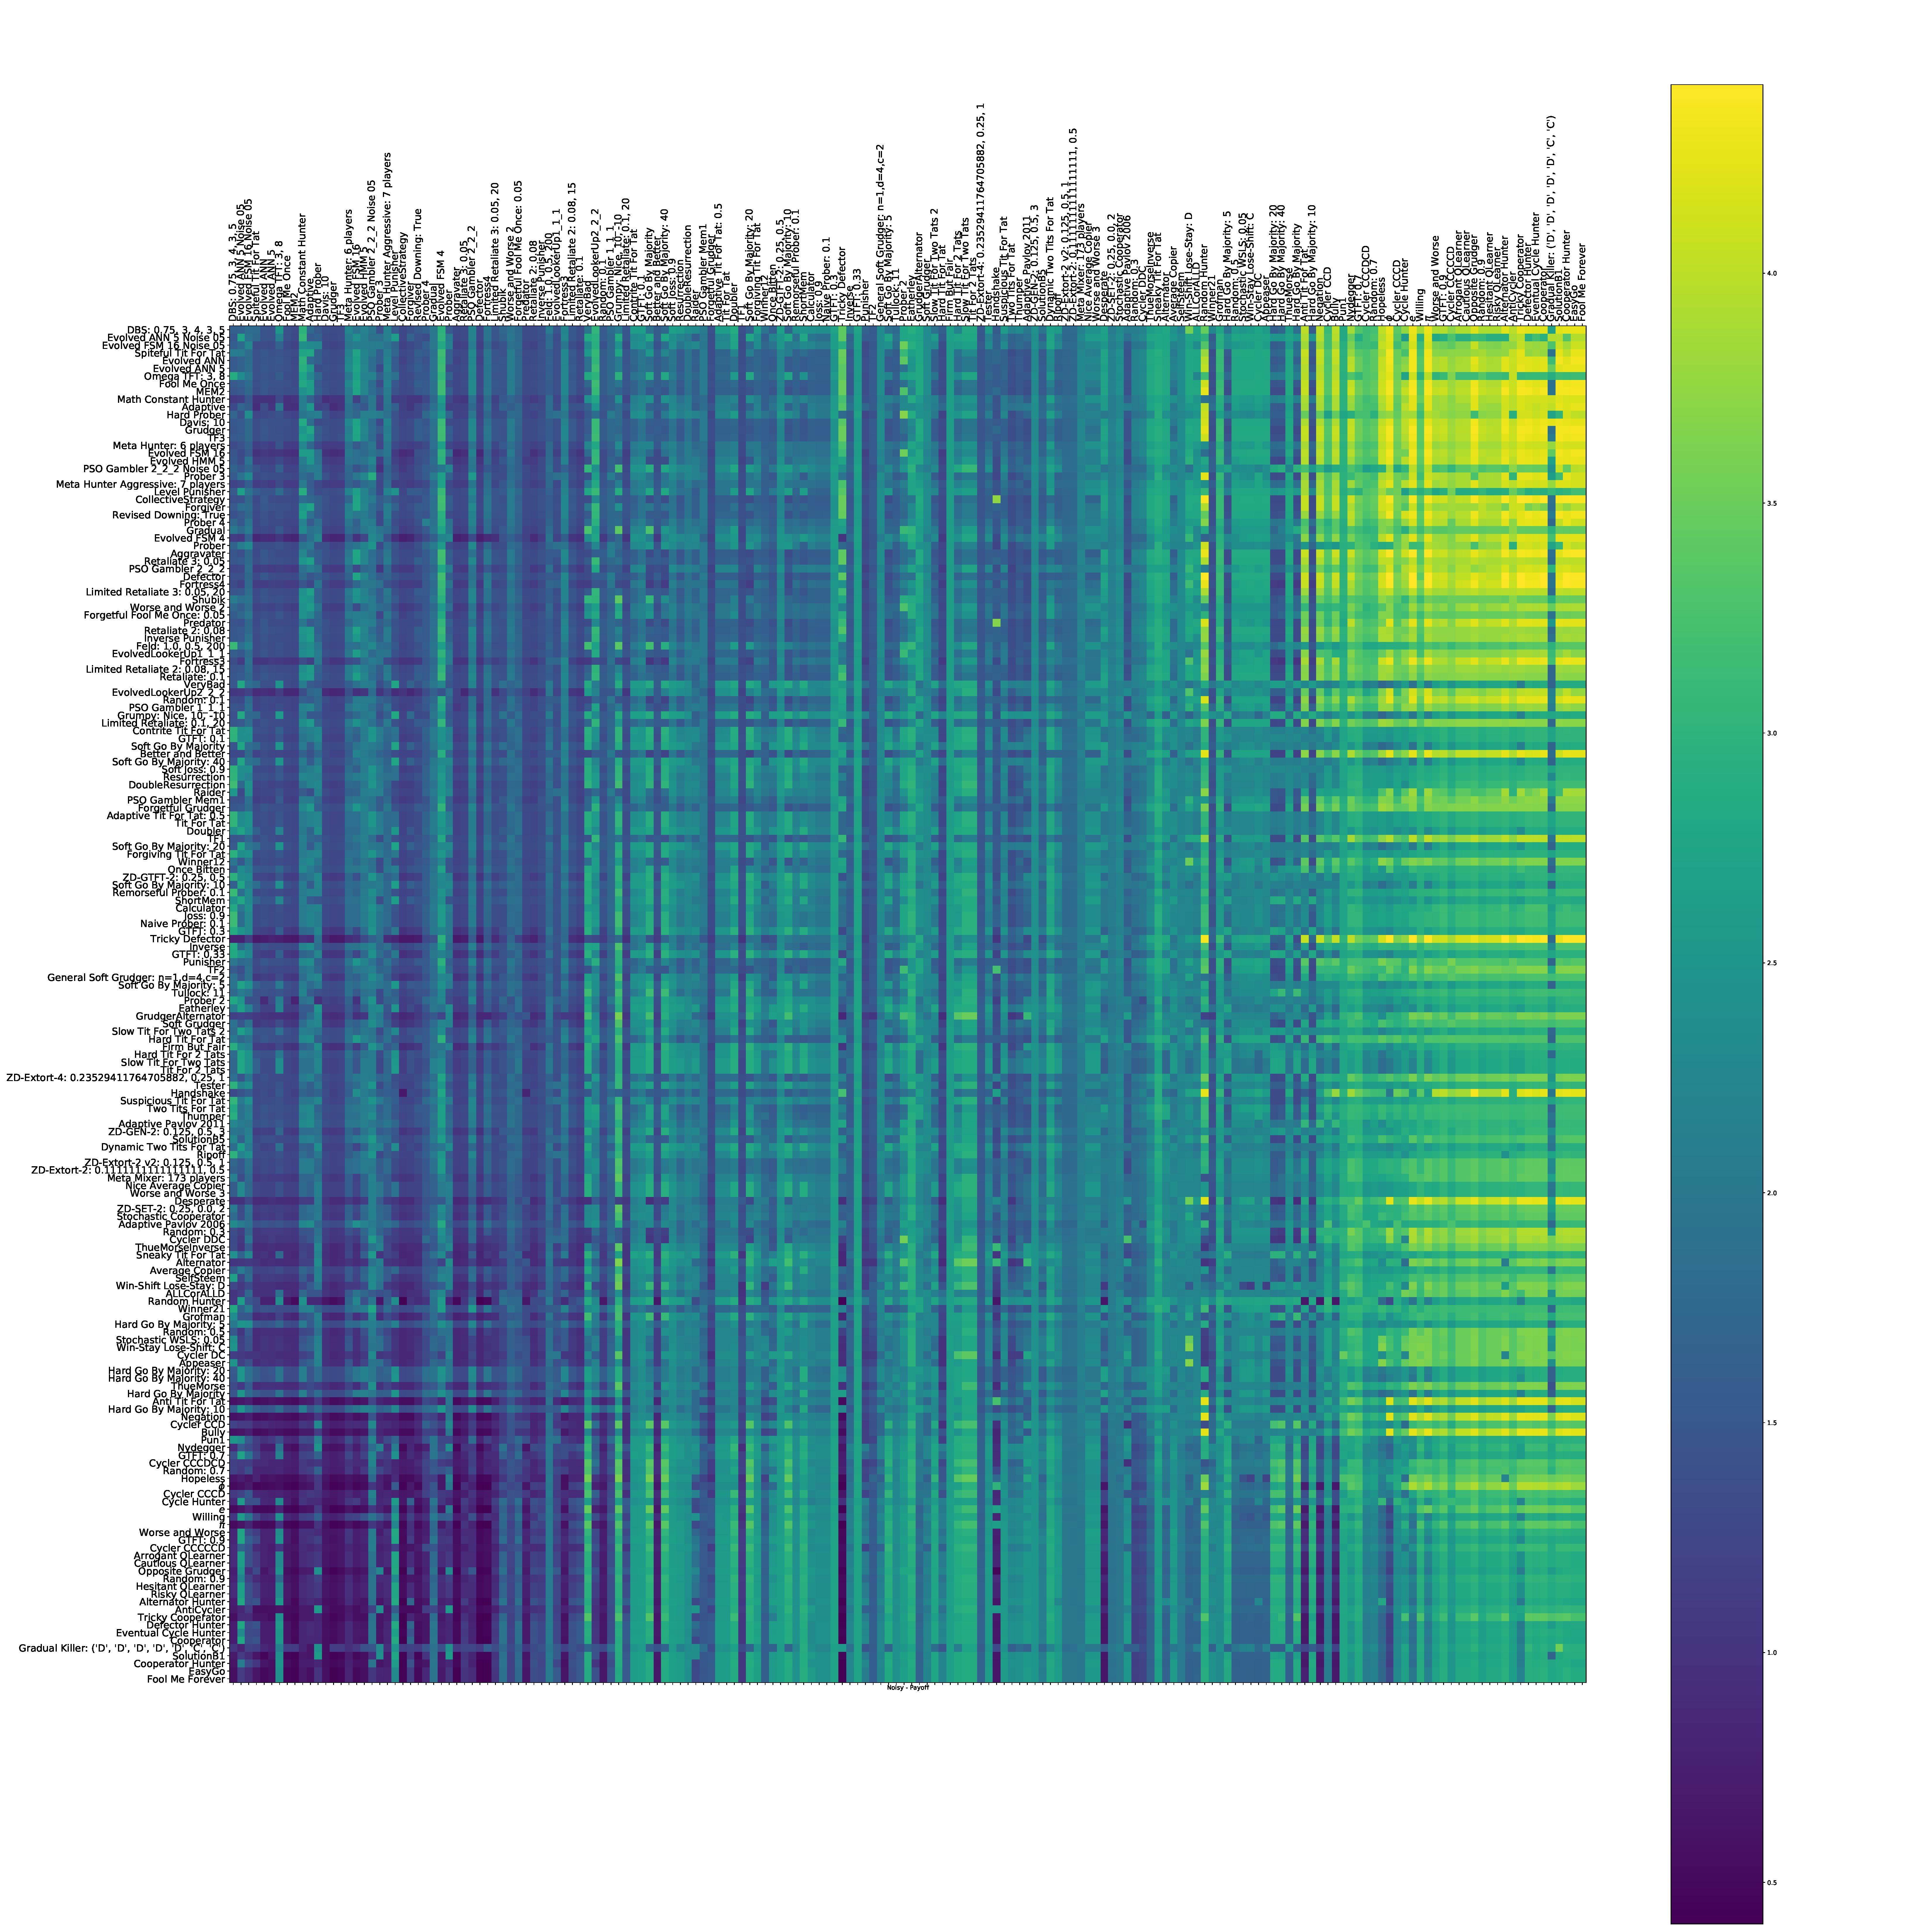
\includegraphics[width=\paperwidth]{plots/Noisy_payoff.pdf}
    \caption{Pairwise Match results for the Noisy Tournament}
\end{figure}

Using the method of fingerprinting described in \cite{ashlock2008fingerprinting}
\cite{ashlock2009fingerprint}, we can compare
strategies. For the top performing noisy strategies there is a striking similarity
in the fingerprints.

\begin{figure}[!hbtp]
    \centering
    \begin{subfigure}[t]{.3\textwidth}
        \centering
        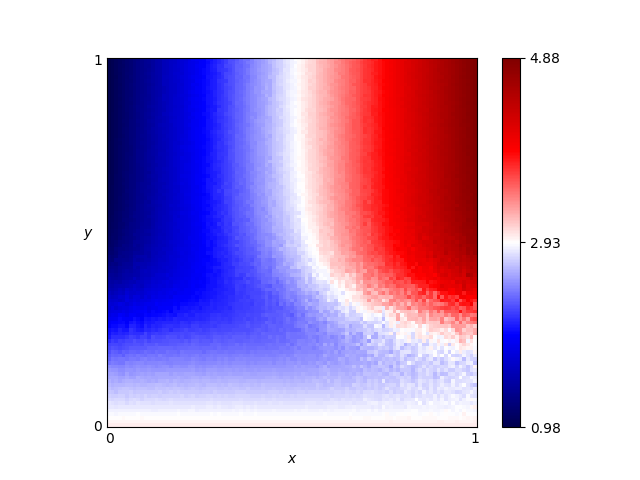
\includegraphics[width=\textwidth]{./plots/DBS.png}
        \caption{Fingerprint for DBS}
    \end{subfigure}%
    ~
    \begin{subfigure}[t]{.3\textwidth}
        \centering
        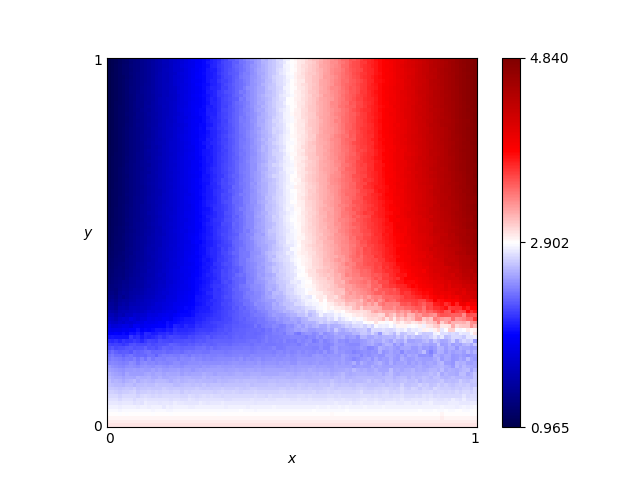
\includegraphics[width=\textwidth]{./plots/Evolved_ANN_5_Noise_05.png}
        \caption{Fingerprint for Evolved\_ANN\_5\_Noise\_05}
    \end{subfigure}%
    ~
    \begin{subfigure}[t]{.3\textwidth}
        \centering
        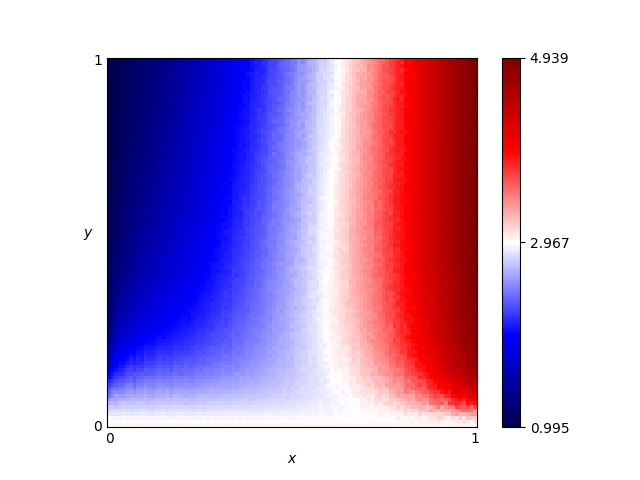
\includegraphics[width=\textwidth]{./plots/Evolved_FSM_16_Noise_05.png}
        \caption{Fingerprint for Evolved\_FSM\_16\_Noise\_05}
    \end{subfigure}%

    \caption{Comparison of Fingerprints for Noisy Tournament Top 3}
    \label{fig:comparison_fingerprint_noisy}
\end{figure}



\section{Methods}

We trained a variety of strategies using evolutionary algorithms, and in the
case of PSO Gambler particle swarm algorithms. The evolutionary algorithms
used standard techniques, varying strategies by mutation and crossover, and
evaluating the performance against each opponent for many repetitions. The
best performing strategies in each generation are persisted, variants created,
and objective functions computed again. This process continues for approximately
200 generations or until strategies no longer improve significantly.

% Todo: Diagram with ANN training performance?

All training code is available on github. There are objective functions for
* total payoff
* total payoff difference
* total Moran process wins (fixation probability)

New strategies can be easily trained with variations including noise, spatial
structure, and probabilistically ending matches.

\section{Discussion}

The tournament results indicate that pre-trained strategies are generally better
than human designed strategies at maximizing payoff against a diverse set of
opponents. A simple evolutionary algorithm produces strategies based on multiple
standard machine learning techniques that are able to achieve a higher mean
score than any other known opponent in a standard tournament. Most of the trained
strategies use multiple rounds of the history of play (some using all of it) and
outperform memory-one strategies (though the trained memory one strategy performs
well). The generic structure of the trained strategy did not appear to be
critical -- strategies based on lookup tables, finite state machines, and stochastic
variants all performed well. Single layer neural networks also performed well
though these had some aspect of human involvement in the selection of features.
The success of the other strategy types suggests that a deeper network that
incorporates feature engineering would likely also perform well.

In opposition to historical tournament results and community folklore,
our results show that complex strategies can be very effective for the
IPD. It is not the complexity of strategies that is disadvantageous; rather that directly
designing a broadly effective strategy is no easy task. Of all the human-designed
strategies in the library, only DBS consistently performs well, and it is
substantially more complex than traditional tournament winners like TFT, OmegaTFT,
and zero determinant strategies. Furthermore, dealing with noise is difficult
for most strategies. Two strategies designed specifically to account for noise,
DBS and OmegaTFT, perform well and only DBS performs better than our trained
strategies.

Of the strategies trained to maximize their mean score all are generally
cooperative, not defecting until the opponent defects. Maximizing for individual
performance across a collection of opponents leads to mutual cooperation despite
the fact that mutual cooperation is an unstable equilibrium for the prisoner's
dilemma. Specifically we note that the reinforcement learning process for maximizing
payout does not
lead to exploitative zero determinant strategies, which may be a result of the
collection of training strategies, many of which retaliate harshly.

Finally, we note that as the library grows, the top performing strategies
sometimes shuffle, and are not retrained regularly. Most of the strategies were
trained on an earlier version of the library (v2.2.0) that did not include DBS
and several other opponents. The precise parameters that are optimal will depend
on the pool of opponents. Moreover we have not extensively trained strategies to
determine the minimum parameters that are sufficient -- neural networks with
fewer nodes and features and finite state machines with fewer states may suffice.
See \cite{ashlock2013impact} for discussion of resource availability for IPD strategies.


Future work:
* spatial tournaments and other variants
* Additional strategy archetypes by the Ashlocks, e.g. function stacks, binary
decision players
* further refine features and training parameters

% TODO: Full strategy list

% TODO: author contributions

\section*{Acknowledgements}

This work was performed using the computational facilities of the Advanced
Research Computing @ Cardiff (ARCCA) Division, Cardiff University.

\printbibliography

\end{document}
